\documentclass[tikz,border=3mm]{standalone}
\usepackage{pgfplots}
\usetikzlibrary{positioning}
\tikzset{
    mybox/.style={
        draw,
        thick,
        align=center,
        fill=white,
        inner sep=0.2em
    }
}
\begin{document}
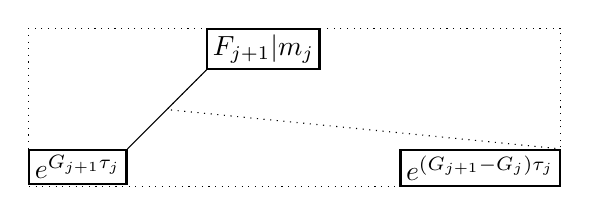
\begin{tikzpicture}[transform shape]
    \node[mybox] (f) {$F_{j+1}|m_j$};
    \node[mybox, below left=of f] (g) {$e^{G_{j+1}\tau_j}$};
    \node[mybox, below right=of f] (h) {$e^{(G_{j+1}-G_j)\tau_j}$};
    \draw[dotted] (current bounding box.north west) rectangle (current bounding box.south east);
    \draw (f.south west) -- (g.north east) coordinate[pos=0.5] (aux);
    \draw[dotted] (f.south west) -- (aux) -- (h.north east);
\end{tikzpicture}
\end{document}